% Author: Izaak Neutelings (October 2020)
% Instructions: To compile, include data files from
%   https://github.com/IzaakWN/CodeSnippets/tree/master/LaTeX/TikZ/physics/dynamics_pendulum
% Other sources:
%   https://www.scielo.br/scielo.php?script=sci_arttext&pid=S1806-11172007000400024
%   https://www.researchgate.net/publication/262746594_Exact_solution_for_the_nonlinear_pendulum
%   https://tex.stackexchange.com/questions/545590/phase-portrait-of-van-der-pol-oscillator-with-pgfplots
%   http://matlab.cheme.cmu.edu/2011/08/09/phase-portraits-of-a-system-of-odes/
\documentclass[border=3pt,tikz]{standalone}
\usepackage{physics}
\usepackage{siunitx}
\sisetup{detect-all} % to allow \pi in \SI
\usepackage{tikz,pgfplots}
\usepackage[outline]{contour} % glow around text
\usetikzlibrary{calc}
\usetikzlibrary{angles,quotes} % for pic
\usetikzlibrary{arrows.meta}
\tikzset{>=latex} % for LaTeX arrow head
\contourlength{1.2pt}

\colorlet{xcol}{blue!70!black}
\colorlet{vcol}{green!60!black}
\colorlet{myred}{red!70!black}
\colorlet{myblue}{blue!70!black}
\colorlet{mygreen}{green!70!black}
\colorlet{mydarkred}{myred!70!black}
\colorlet{mydarkblue}{myblue!60!black}
\colorlet{mydarkgreen}{mygreen!60!black}
\colorlet{acol}{red!50!blue!80!black!80}
\tikzstyle{CM}=[red!40!black,fill=red!80!black!80]
\tikzstyle{xline}=[xcol,thick,smooth]
\tikzstyle{mass}=[line width=0.6,red!30!black,fill=red!40!black!10,rounded corners=1,
                  top color=red!40!black!20,bottom color=red!40!black!10,shading angle=20]
\tikzstyle{faded mass}=[dashed,line width=0.1,red!30!black!40,fill=red!40!black!10,rounded corners=1,
                        top color=red!40!black!10,bottom color=red!40!black!10,shading angle=20]
\tikzstyle{rope}=[brown!70!black,very thick,line cap=round]
\def\rope#1{ \draw[black,line width=1.4] #1; \draw[rope,line width=1.1] #1; }
\tikzstyle{force}=[->,myred,very thick,line cap=round]
\tikzstyle{velocity}=[->,vcol,very thick,line cap=round]
\tikzstyle{Fproj}=[force,myred!40]
\tikzstyle{myarr}=[-{Latex[length=3,width=2]},thin]
\def\tick#1#2{\draw[thick] (#1)++(#2:0.12) --++ (#2-180:0.24)}
\DeclareMathOperator{\sn}{sn}
\DeclareMathOperator{\cn}{cn}
\DeclareMathOperator{\dn}{dn}
\def\N{80} % number of samples in plots


\begin{document}


% PENDULUM
\def\L{2.8}  % string length
\def\ang{28} % angle string
\def\R{0.25} % ball radius
\def\F{1.0}  % force magnitude
\begin{tikzpicture}
  \message{^^JPendulum}
  \coordinate (M) at (\ang-90:\L);
  \coordinate (M') at (0,-\L);
  \coordinate (O) at (0,0);
  \coordinate (B) at (0,-\L-2.2*\R);
  \coordinate (FT) at ($(M)+(90+\ang:{\F*cos(\ang)+\R})$);
  \coordinate (FG) at ($(M)+(-90:{\F+\R})$);
  \coordinate (FGx) at ($(M)+(-90+\ang:{0.55*\F+\R})$);
  \coordinate (MA) at ($(M)+(180+\ang:{\F*sin(\ang)+\R})$);
  %\draw[faded mass] (M') circle(\R);
  \draw[<->] (M)++(\ang-32:0.2*\L) node[below right=-1,scale=0.9] {$x$}
    --++ (\ang:0.17*\L) --++ (90+\ang:0.17*\L) node[above right=-1,scale=0.9] {$y$};
  \draw[dashed] (O) -- (B);
  %\draw[dashed,myred!60!black] (MA) -- (FG);
  \draw[dashed,myred!60!black] (M) -- (FGx);
  \draw[dashed] (-90+\ang+10:\L) arc(-90+\ang+10:-110:\L) (B);
  \rope{(O) -- (M)} \path (O) -- (M) node[midway,above right=-1] {$L$};
  \fill[black] (O) circle(0.04);
  \draw[force] (M) -- (FT) node[midway,left=0] {$\vb{T}$};
  \draw[force] (M) -- (FG) node[right=0] {$m\vb{g}$};
  \draw[force,acol] (M) -- (MA) node[right=2,below=0] {$m\vb{a}$}; %{\contour{white}{$m\vb{a}$}};
  \draw[mass] (M) circle(\R) node {$m$};
  \draw pic[myarr,"$\theta$",xcol,draw=xcol,angle radius=22,angle eccentricity=1.30] {angle=B--O--M}; %_\text{max}
  \draw pic[myarr,"$\theta$",xcol,draw=xcol,angle radius=14,angle eccentricity=1.45] {angle=FG--M--FGx};
\end{tikzpicture}


% PENDULUM FORCES - ma
\begin{tikzpicture}
  \message{^^JPendulum forces}
  \def\F{1.4}  % force magnitude
  \coordinate (O) at (0,0);
  \coordinate (FT) at (90+\ang:{\F*cos(\ang)});
  \coordinate (FG) at (-90:\F);
  \coordinate (FGx) at (-90+\ang:{0.7*\F});
  \coordinate (MA) at (180+\ang:{\F*sin(\ang)});
  \draw[dashed,myred!60!black] (O) -- (FGx);
  \draw[dashed,myred!60!black] (MA) -- (FG);
  \draw[force] (O) -- (FT) node[midway,above right=-2] {$\vb{T}$};
  \draw[force] (O) -- (FG) node[right=0] {$m\vb{g}$};
  \draw[force,acol] (O) -- (MA) node[left=0] {$m\vb{a}$};
  \draw pic[myarr,"$\theta$",xcol,draw=xcol,angle radius=14,angle eccentricity=1.45] {angle=FG--O--FGx};
\end{tikzpicture}


% PENDULUM FORCES
\begin{tikzpicture}
  \message{^^JPendulum forces}
  \def\F{1.4}  % force magnitude
  \coordinate (O) at (0,0);
  \coordinate (FT) at (90+\ang:{\F*cos(\ang)});
  \coordinate (FG) at (-90:\F);
  \coordinate (FGx) at (-90+\ang:{\F*cos(\ang)});
  \coordinate (FGy) at (180+\ang:{\F*sin(\ang)});
  \draw[dashed,myred!60!black] (FGy) -- (FG); %-- (FGx);
  \draw[force] (O) -- (FT) node[midway,above right=-2] {$\vb{T}$};
  \draw[Fproj] (O) -- (FGy) node[pos=0.4,above left=-3,scale=0.86] {$mg\sin\theta$};
  \draw[Fproj] (O) -- (FGx) node[pos=0.5,above right=-3,scale=0.86] {$mg\cos\theta$};
  \draw[force] (O) -- (FG) node[right=0] {$m\vb{g}$};
  \draw pic[myarr,"$\theta$",xcol,draw=xcol,angle radius=14,angle eccentricity=1.45] {angle=FG--O--FGx};
\end{tikzpicture}


%% PENDULUM 
%\begin{tikzpicture}
%  \coordinate (M) at (0,-\L);
%  \coordinate (O) at (0,0);
%  \rope{(O) -- (M)} \path (O) -- (M) node[midway,above right=-2] {$L$};
%  \fill[black] (O) circle(0.04);
%  \draw[velocity] (M)++(-\R,0) --++ (-2.7*\R,0) node[above=0] {$\vb{v}$};
%  \draw[mass] (M) circle(\R) node {$m$};
%\end{tikzpicture}


% PHYSICAL PENDULUM
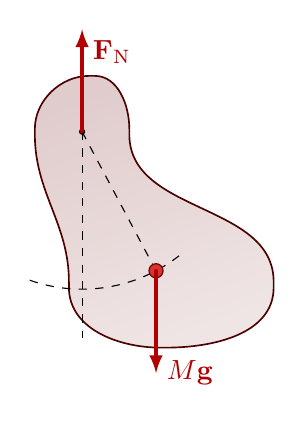
\begin{tikzpicture}
  \message{^^JPhysical pendulum}
  \def\L{2.0}  % string length
  \def\ang{28} % angle string
  \def\R{0.25} % ball radius
  \def\F{1.3}  % force magnitude
  \coordinate (M) at (\ang-90:\L);
  \coordinate (R) at (\ang-90:1.1*\L);
  \coordinate (M') at (0,-\L);
  \coordinate (O) at (0,0);
  \coordinate (B) at (0,-\L-2.5*\R);
  \coordinate (FT) at (90:\F);
  \coordinate (FG) at ($(M)+(-90:\F)$);
  \coordinate (FGx) at ($(M)+(-90+\ang:{0.55*\F+\R})$);
  \coordinate (MA) at ($(M)+(180+\ang:{\F*sin(\ang)+\R})$);
  \draw[mass]
    (180:0.3*\L) to[out=90,in=180] (80:0.36*\L) to[out=0,in=90] (0:0.3*\L) to[out=-90,in=90]
    ($(R)+(0:0.7*\L)$) to[out=-90,in=0] ($(R)+(-90:0.4*\L)$) to[out=180,in=-90] ($(R)+(-180:0.6*\L)$) to[out=90,in=-90] cycle; %node {$m$};
  \draw[dashed] (O) -- (B);
  \draw[dashed] (O) -- (M);
  %\draw[dashed,myred!60!black] (MA) -- (FG);
  \draw[dashed] (-90+\ang+10:\L) arc(-90+\ang+10:-110:\L) (B);
  \fill[black] (O) circle(0.04);
  \draw[CM] (M) circle(0.09);
  \draw[force] (O) -- (FT) node[below right=0] {$\vb{F}_\mathrm{N}$};
  \draw[force] (M) -- (FG) node[right=0] {$M\vb{g}$};
%  \draw[force,acol] (M) -- (MA) node[right=2,below=0] {$m\vb{a}$}; %{\contour{white}{$m\vb{a}$}};
%  \draw pic[myarr,"$\theta$",xcol,draw=xcol,angle radius=22,angle eccentricity=1.30] {angle=B--O--M}; %_\text{max}
%  \draw pic[myarr,"$\theta$",xcol,draw=xcol,angle radius=14,angle eccentricity=1.45] {angle=FG--M--FGx};
\end{tikzpicture}


%% EXACT SOLUTION
%% Other sources:
%%   https://www.scielo.br/scielo.php?script=sci_arttext&pid=S1806-11172007000400024
%%   https://www.researchgate.net/publication/262746594_Exact_solution_for_the_nonlinear_pendulum
%%   https://tex.stackexchange.com/questions/545590/phase-portrait-of-van-der-pol-oscillator-with-pgfplots
%%   http://matlab.cheme.cmu.edu/2011/08/09/phase-portraits-of-a-system-of-odes/
%% Instructions to compile this part of the code:
%%   These curves were generated numerically with these MATLAB scripts:
%%     https://github.com/IzaakWN/CodeSnippets/tree/master/LaTeX/TikZ/physics/dynamics_pendulum
%%   To compile this part of the code, the curves need to be loaded via external txt files.
%%   To download the txt files from GitHub via the command line, do e.g.
%%     wget https://github.com/IzaakWN/CodeSnippets/raw/master/LaTeX/TikZ/physics/dynamics_pendulum.zip
%%     unzip dynamics_pendulum.zip
%%   or
%%     svn checkout https://github.com/IzaakWN/CodeSnippets/trunk/LaTeX/TikZ/physics/dynamics_pendulum/data ./dynamics_pendulum/data
%\begin{tikzpicture}
%  \message{^^JPendulum exact solution}
%  \def\xmax{7.0}  % max x axis
%  \def\ymax{1.4}  % max y axis
%  \def\A{3.1*\ys} % amplitude, theta0 = 3.1 ~ 178°
%  \def\B{2.4*\ys} % amplitude, theta0 = 2.4 ~ 140°
%  \def\C{0.6*\ys} % amplitude, theta0 = 0.6 ~ 34.4°
%  \pgfmathsetmacro\Tb{\xmax/2.97}      % period, theta0 = 2.4 ~ 140°, T/T0 ~ 1.5602
%  \pgfmathsetmacro\Ta{\Tb*3.35/1.56}   % period, theta0 = 3.1 ~ 178°, T/T0 ~ 3.3485
%  \pgfmathsetmacro\Tc{\Tb*1.023/1.56}  % period, theta0 = 0.6 ~ 34.4°, T/T0 ~ 1.0230
%  \pgfmathsetmacro\xs{\Ta/(2*pi*3.35)} % xscale, note data uses T = 2*pi, omega0 = 1
%  \pgfmathsetmacro\ys{\ymax*0.28}      % yscale
%  
%  % AXIS
%  \draw[->,thick] (0,-\ymax) -- (0,\ymax+0.2) node[above=-3] {$\theta$ [rad]};
%  \draw[->,thick] (-0.2,0) -- (\xmax+0.05,0) node[right=-1] {$t$ [s]};
%  \draw[mydarkblue!30,dashed]
%    (0, pi*\ys) --++ (0.90*\xmax,0)
%    node[right=1,scale=0.8] {$ \pi\,\si{rad}= \SI{180}{\degree}$}
%    (0,-pi*\ys) --++ (0.84*\xmax,0)
%    node[right=1,scale=0.8] {$-\pi\,\si{rad}=-\SI{180}{\degree}$};
%  
%  % PLOT REAL PENDULUM
%  \begin{axis}[
%      axis lines=none,anchor=origin,x=1cm,y=1cm, % coincide with TikZ coordinates
%      xmin=0,xmax=0.94*\xmax/\xs,xscale=\xs,
%      y filter/.code={\pgfmathparse{\ys*\pgfmathresult}}
%    ]
%    \addplot[xline,mygreen] table {dynamics_pendulum/data/pendulum-0p6.txt};
%    \addplot[xline,myred] table {dynamics_pendulum/data/pendulum-2p4.txt};
%    \addplot[xline,xcol] table {dynamics_pendulum/data/pendulum-3p1.txt};
%  \end{axis}
%  
%  % PLOT APPROXIMATION
%  \draw[xline,mydarkgreen,thin,dashed,samples=\N,smooth,variable=\x,domain=0:0.94*\xmax]
%    plot(\x,{\C*cos(360/\Tc*\x)});
%  \draw[xline,mydarkred,thin,dashed,samples=\N,smooth,variable=\x,domain=0:0.94*\xmax]
%    plot(\x,{\B*cos(360/\Tb*\x)});
%  \draw[xline,mydarkblue,thin,dashed,samples=\N,smooth,variable=\x,domain=0:0.94*\xmax]
%    plot(\x,{\A*cos(360/\Ta*\x)});
%  
%  % TICKS
%  \tick{0, \A}{0} node[above=1,left=-1,scale=0.9,mydarkblue] {3.1}; %\SI{3.1}{\degree}
%  \tick{0, \B}{0} node[below=0.5,left=-1,scale=0.9,mydarkred] {2.4};
%  \tick{0, \C}{0} node[below=0.5,left=-1,scale=0.9,mydarkgreen] {0.6};
%  \tick{0,-\A}{0} node[left=-1,scale=0.9,mydarkblue] {$-3.1$};
%  \tick{\Tb,0}{90} node[below,scale=0.9,mydarkred] {$T(2.4)$};
%  \tick{2*\Tb,0}{90} node[below,scale=0.9] {$2\color{mydarkred}{T(2.4)}$};
%  
%\end{tikzpicture}
%
%
%% EXACT SOLUTION - angular velocity
%\begin{tikzpicture}
%  \message{^^JPendulum exact solution - dtheta/dt}
%  \def\xmax{7.0}   % max x axis
%  \def\ymax{1.4}   % max y axis
%  \def\wmax{2*\ys} % yscale
%  \pgfmathsetmacro\Ta{\xmax/2.97}      % period, theta0 = 2.4 ~ 140°, T/T0 ~ 1.5602
%  \pgfmathsetmacro\Tb{\Ta*3.35/1.56}   % period, theta0 = 3.1 ~ 178°, T/T0 ~ 3.3485
%  \pgfmathsetmacro\xs{\Tb/(2*pi*3.35)} % xscale, note data uses T = 2*pi, omega0 = 1
%  \pgfmathsetmacro\ys{\ymax*0.44}      % yscale
%  \pgfmathsetmacro\A{2*sin(deg(2.4/2))*\ys}  % amplitude, theta0 = 2.4 ~ 140°
%  \pgfmathsetmacro\B{2*sin(deg(3.1/2))*\ys}  % amplitude, theta0 = 3.1 ~ 178°
%  
%  % AXIS
%  \draw[->,thick] (0,-\ymax) -- (0,\ymax+0.2) node[above=-3] {$\dot{\theta}$ [rad/s]};
%  \draw[->,thick] (-0.2,0) -- (\xmax+0.05,0) node[right=-1] {$t$ [s]};
%  \draw[mydarkblue!30,dashed]
%    (0, \wmax) --++ (0.9*\xmax,0) %node[right=1,scale=0.8] {$ \SI{\pi}{rad}= \SI{180}{\degree}$}
%    (0,-\wmax) --++ (0.9*\xmax,0); %node[right=1,scale=0.8] {$-\SI{\pi}{rad}=-\SI{180}{\degree}$};
%  
%  % PLOT REAL PENDULUM
%  \begin{axis}[
%      axis lines=none,anchor=origin,x=1cm,y=1cm, % coincide with TikZ coordinates
%      xmin=0,xmax=0.94*\xmax/\xs,xscale=\xs,
%      y filter/.code={\pgfmathparse{\ys*\pgfmathresult}}
%    ]
%    \addplot[xline,myred]
%      table[y index=2] {dynamics_pendulum/data/pendulum-2p4.txt};
%    \addplot[xline,xcol]
%      table[y index=2] {dynamics_pendulum/data/pendulum-3p1.txt};
%  \end{axis}
%  
%  % PLOT APPROXIMATION
%  \draw[xline,mydarkred,thin,dashed,samples=\N,smooth,variable=\x,domain=0:0.94*\xmax]
%    plot(\x,{-\A*sin(360/\Ta*\x)});
%  \draw[xline,mydarkblue,thin,dashed,samples=\N,smooth,variable=\x,domain=0:0.94*\xmax]
%    plot(\x,{-\B*sin(360/\Tb*\x)});
%  
%  % TICKS
%  \tick{0, \wmax}{0} node[left=-2,scale=0.9] {$2\omega_0$};
%  \tick{0,-\wmax}{0} node[left=-2,scale=0.9] {$-2\omega_0$};
%  \tick{\Ta,0}{90} node[below,scale=0.9] {\contour{white}{$\color{mydarkred}{T(2.4)}$}};
%  \tick{2*\Ta,0}{90} node[below,scale=0.9] {\contour{white}{$2\color{mydarkred}{T(2.4)}$}};
%  
%\end{tikzpicture}
%
%
%% EXACT SOLUTION
%\begin{tikzpicture}
%  \message{^^JPendulum exact solution (normalized)}
%  \def\xmax{7.0}  % max x axis
%  \def\ymax{1.4}  % max y axis
%  \def\A{3.1*\ys} % amplitude, theta0 = 3.1 ~ 178°
%  \def\B{2.4*\ys} % amplitude, theta0 = 2.4 ~ 140°
%  \def\C{1.6*\ys} % amplitude, theta0 = 1.6 ~ 91.7
%  \pgfmathsetmacro\T{0.95*\xmax/2} % period
%  \pgfmathsetmacro\ys{\ymax*0.28}  % yscale
%  
%  % AXIS
%  \draw[->,thick] (0,-\ymax) -- (0,\ymax+0.2) node[above=-3] {$\theta$ [rad]};
%  \draw[->,thick] (-0.2,0) -- (\xmax+0.05,0) node[right=-1] {$t$ [s]};
%  \draw[mydarkblue!30,dashed]
%    (0, pi*\ys) --++ (0.98*\xmax,0) node[right=1,scale=0.8] {$ \pi\,\si{rad}= \SI{180}{\degree}$}
%    (0,-pi*\ys) --++ (0.90*\xmax,0) node[right=1,scale=0.8] {$-\pi\,\si{rad}=-\SI{180}{\degree}$};
%  
%  % PLOT REAL PENDULUM
%  \begin{axis}[
%      axis lines=none,anchor=origin,x=1cm,y=1cm, % coincide with TikZ coordinates
%      xmin=0,xscale=\T, %0.94*7/3, %xmax=0.94*\xmax/\xs,
%      y filter/.code={\pgfmathparse{\ys*\pgfmathresult}}
%    ]
%    \addplot[xline,mygreen] table {dynamics_pendulum/data/pendulum-1p6_norm.txt};
%    \addplot[xline,myred] table {dynamics_pendulum/data/pendulum-2p4_norm.txt};
%    \addplot[xline,xcol] table {dynamics_pendulum/data/pendulum-3p1_norm.txt};
%  \end{axis}
%  
%  % PLOT APPROXIMATION
%  \draw[xline,mydarkblue,thin,dashed,samples=\N,smooth,variable=\x,domain=0:0.94*\xmax]
%    plot(\x,{\A*cos(360/\T*\x)});
%  \draw[xline,mydarkred,thin,dashed,samples=\N,smooth,variable=\x,domain=0:0.94*\xmax]
%    plot(\x,{\B*cos(360/\T*\x)});
%  \draw[xline,mydarkgreen,thin,dashed,samples=\N,smooth,variable=\x,domain=0:0.94*\xmax]
%    plot(\x,{\C*cos(360/\T*\x)});
%  
%  % TICKS
%  \tick{0, \A}{0} node[above=1,left=-1,scale=0.9] {\color{mydarkblue}{3.1}};
%  \tick{0, \B}{0} node[below=0.5,left=-1,scale=0.9] {\color{mydarkred}{2.4}};
%  \tick{0, \C}{0} node[below=0.5,left=-1,scale=0.9] {\color{mydarkgreen}{1.6}};
%  \tick{0,-\A}{0} node[left=-1,scale=0.9] {\color{mydarkblue}{$-3.1$}};
%  \tick{\T,0}{90} node[below,scale=0.9] {$T$};
%  \tick{2*\T,0}{90} node[below,scale=0.9] {$2T$};
%  
%\end{tikzpicture}
%
%
%% EXACT SOLUTION - angular velocity
%\begin{tikzpicture}
%  \message{^^JPendulum exact solution - dtheta/dt (normalized)}
%  \def\xmax{7.0}   % max x axis
%  \def\ymax{1.4}   % max y axis
%  \def\wmax{2*\ys} % yscale
%  \pgfmathsetmacro\T{0.95*\xmax/2} % period  
%  \pgfmathsetmacro\ys{\ymax*0.44}  % yscale
%  \pgfmathsetmacro\A{2*sin(deg(3.1/2))*\ys}  % amplitude, theta0 = 3.1 ~ 178°
%  \pgfmathsetmacro\B{2*sin(deg(2.4/2))*\ys}  % amplitude, theta0 = 2.4 ~ 140°
%  \pgfmathsetmacro\C{2*sin(deg(1.6/2))*\ys}  % amplitude, theta0 = 1.6 ~ 91.7°
%  
%  % AXIS
%  \draw[->,thick] (0,-\ymax) -- (0,\ymax+0.2) node[above=-3] {$\dot{\theta}$ [rad/s]};
%  \draw[->,thick] (-0.2,0) -- (\xmax+0.05,0) node[right=-1] {$t$ [s]};
%  \draw[mydarkblue!30,dashed]
%    (0, \wmax) --++ (0.9*\xmax,0) %node[right=1,scale=0.8] {$ \SI{\pi}{rad}= \SI{180}{\degree}$}
%    (0,-\wmax) --++ (0.9*\xmax,0); %node[right=1,scale=0.8] {$-\SI{\pi}{rad}=-\SI{180}{\degree}$};
%  
%  % PLOT REAL PENDULUM
%  \begin{axis}[
%      axis lines=none,anchor=origin,x=1cm,y=1cm, % coincide with TikZ coordinates
%      xmin=0,xscale=\T,
%      y filter/.code={\pgfmathparse{\ys*\pgfmathresult}}
%    ]
%    \addplot[xline,xcol]
%      table[y index=2] {dynamics_pendulum/data/pendulum-3p1_norm.txt};
%    \addplot[xline,myred]
%      table[y index=2] {dynamics_pendulum/data/pendulum-2p4_norm.txt};
%    \addplot[xline,mygreen]
%      table[y index=2] {dynamics_pendulum/data/pendulum-1p6_norm.txt};
%  \end{axis}
%  
%  % PLOT APPROXIMATION
%  \draw[xline,mydarkblue,thin,dashed,samples=\N,smooth,variable=\x,domain=0:0.94*\xmax]
%    plot(\x,{-\A*sin(360/\T*\x)});
%  \draw[xline,mydarkred,thin,dashed,samples=\N,smooth,variable=\x,domain=0:0.94*\xmax]
%    plot(\x,{-\B*sin(360/\T*\x)});
%  \draw[xline,mydarkgreen,thin,dashed,samples=\N,smooth,variable=\x,domain=0:0.94*\xmax]
%    plot(\x,{-\C*sin(360/\T*\x)});
%  
%  % LABELS
%  \node[above=0,scale=0.8,mydarkblue] at (0.78*\T,0.99*\A) {$\theta_0=3.1$};
%  \node[right,scale=0.8,mydarkred] at (0.81*\T,0.88*\B) {\contour{white}{$\theta_0=2.4$}};
%  \node[right,scale=0.8,mydarkgreen] at (0.96*\T,0.4*\C) {$\theta_0=1.6$};
%  
%  % TICKS
%  \tick{0, \wmax}{0} node[left=-2,scale=0.9] {$2\omega_0$};
%  \tick{0,-\wmax}{0} node[left=-2,scale=0.9] {$-2\omega_0$};
%  \tick{\T,0}{90} node[left=2,below,scale=0.9] {$T$};
%  \tick{2*\T,0}{90} node[below,scale=0.9] {$2\color{mydarkred}{T}$};
%  
%\end{tikzpicture}
%
%
%% EXACT SOLUTION - T/T0
%% https://en.wikipedia.org/wiki/Pendulum_(mathematics)
%\begin{tikzpicture}[xscale=1.1]
%  \message{^^JPendulum exact solution period (closed/bounded)}
%  \def\xmax{4.1}   % max x axis
%  \def\ymax{3.2}   % max y axis
%  \def\ys{0.82}    % yscale
%  \def\xs{1.02}    % xscale
%  \def\yz{\ys*0.4} % y zero
%  \def\xtick#1{\draw[thick] (#1)++(0,0.11) --++ (0,-0.22)}
%  \def\ytick#1{\draw[thick] (#1)++(0.1,0) --++ (-0.2,0)}
%  
%  % AXIS
%  \draw[->,thick]
%    (0,\yz-0.1*\ymax) -- (0,\ymax+0.1) node[below=3,left=1] {$\dfrac{T}{T_0}$};
%  \draw[->,thick]
%    (-0.1*\ymax,\yz) -- (\xmax,\yz) node[right=3,below=0] {$\theta_0$ [rad]};
%  \draw[dashed] (\xs*pi,\yz) --++ (0,\ymax-\yz);
%  
%  % REAL PENDULUM  
%  \begin{axis}[
%      axis lines=none,anchor=origin,
%      x=1cm,y=1cm,ymin=0,ymax=\ymax,xscale=\xs,
%      y filter/.code={\pgfmathparse{\ys*\pgfmathresult}}
%    ]
%    \addplot[xline]
%      table[x index=0,y index=1] {dynamics_pendulum/data/pendulum_period.txt};
%  \end{axis}
%  
%  % LINES
%  \draw[dashed,mydarkgreen]
%    (0,\ys) --++ (0.82*\xmax,0)
%    node[right=1,scale=0.8,align=left] {small-angle\\[-1mm]approximation};
%  \draw[dashed,mydarkred]
%    (0,\ys*1.18) -| (0.50*pi,\yz);
%  
%  % TICKS
%  \xtick{0.25*\xs*pi,\yz} node[below=1,scale=0.9] {$\dfrac{\pi}{4}$};
%  \xtick{0.50*\xs*pi,\yz} node[below=1,scale=0.9] {$\dfrac{\pi}{2}$};
%  \xtick{0.75*\xs*pi,\yz} node[below=-0.9,scale=0.9] {$\dfrac{3\pi}{4}$};
%  \xtick{     \xs*pi,\yz} node[below=1,scale=0.9] {$\pi$};
%  \ytick{0,\ys} node[below=1.5,left=0,scale=0.9] {1};
%  \ytick{0,\ys*1.18} node[above=3,left=0,scale=0.8,mydarkred] {1.18};
%  \ytick{0,\ys*2} node[left=0,scale=0.9] {2};
%  \ytick{0,\ys*3} node[left=0,scale=0.9] {3};
%  
%\end{tikzpicture}
%
%
%% EXACT SOLUTION - OPEN TRAJECTORY
%\begin{tikzpicture}
%  \message{^^JPendulum exact solution (open/unbounded, normalized)}
%  \def\xmax{7.0} % max x axis
%  \def\ymax{2.8} % max y axis
%  \pgfmathsetmacro\T{0.98*\xmax/2.5} % period
%  \pgfmathsetmacro\ys{\ymax*0.06}    % yscale
%  
%  % AXIS
%  \draw[->,thick] (0,-0.2) -- (0,\ymax+0.2) node[above=-3] {$\theta$ [rad]};
%  \draw[->,thick] (-0.2,0) -- (\xmax+0.25,0) node[right=-1] {$t$ [s]};
%  \draw[mydarkblue!30,dashed,yscale=\ys]
%    (0,pi) --++ (\xmax,0)
%    (0,3*pi) --++ (\xmax,0)
%    (0,5*pi) --++ (\xmax,0);
%  
%  % PLOT REAL PENDULUM
%  \begin{axis}[
%      axis lines=none,anchor=origin,x=1cm,y=1cm, % coincide with TikZ coordinates
%      xmin=0,xscale=\T, %0.94*7/3, %xmax=0.94*\xmax/\xs,
%      y filter/.code={\pgfmathparse{\ys*\pgfmathresult}}
%    ]s
%    \addplot[xline,xcol] table {dynamics_pendulum/data/pendulum_open-2p00000002_norm.txt};
%    \addplot[xline,myred] table {dynamics_pendulum/data/pendulum_open-2p01_norm.txt};
%    \addplot[xline,mygreen] table {dynamics_pendulum/data/pendulum_open-2p6_norm.txt};
%  \end{axis}
%  
%  % LABELS
%  \node[above right=-1,scale=0.8,mydarkblue] at (0.97*\T,\ys*pi) {$\Omega_0/2\omega_0=1.00000001$};
%  %\node[right=2,scale=0.8,mydarkred] at (\T,1.96*\ys*pi) {\contour{white}{$\Omega_0/2\omega_0=1.005$}};
%  \node[below right=0,scale=0.8,mydarkred] at (1.27*\T,3*\ys*pi) {\contour{white}{$\Omega_0/2\omega_0=1.005$}};
%  %\node[below right=-1,scale=0.8,mydarkgreen] at (1.4*\T,3*\ys*pi) {$\Omega_0/2\omega_0=1.3$};
%  \node[below right=0,scale=0.8,mydarkgreen] at (2.01*\T,4.24*\ys*pi) {$\Omega_0/2\omega_0=1.3$};
%  
%  % TICKS
%  \tick{0,pi*\ys}{0} node[left=-1,scale=0.9] {$\pi$};
%  \tick{0,2*pi*\ys}{0} node[left=-1,scale=0.9] {$2\pi$};
%  \tick{0,3*pi*\ys}{0} node[left=-1,scale=0.9] {$3\pi$};
%  \tick{0,4*pi*\ys}{0} node[left=-1,scale=0.9] {$4\pi$};
%  \tick{0,5*pi*\ys}{0} node[left=-1,scale=0.9] {$5\pi$};
%  \tick{\T,0}{90} node[below,scale=0.9] {$T$};
%  \tick{2*\T,0}{90} node[below,scale=0.9] {$2T$};
%  
%\end{tikzpicture}
%
%
%% EXACT SOLUTION - OPEN TRAJECTORIES - T/T0
%% https://en.wikipedia.org/wiki/Pendulum_(mathematics)
%\begin{tikzpicture}
%  \message{^^JPendulum exact solution period (open/unbounded)}
%  \def\xmax{6.1} % max x axis
%  \def\ymax{2.9} % max y axis
%  \def\ys{2.2}   % yscale
%  \def\xs{0.79}   % xscale
%  \def\xtick#1{\draw[thick] (#1)++(0,0.11) --++ (0,-0.22)}
%  \def\ytick#1{\draw[thick] (#1)++(0.12,0) --++ (-0.24,0)}
%  
%  % AXIS
%  \draw[->,thick] (0,-0.1*\ymax) -- (0,\ymax+0.2) node[below=3,left=1] {$\dfrac{T}{T_0}$};
%  \draw[->,thick] (-0.1*\xs*\ymax,0) -- (\xs*\xmax,0) node[right=3,below=0] {$\Omega_0/2\omega_0$};
%  %\draw[dashed] (pi,0) --++ (0,\ymax-0);
%  
%  % UNIFORM MOTION
%  \draw[xline,mydarkgreen,thin,dashed,samples=\N,smooth,variable=\x,domain=\ys/(2.05*\ymax):5]
%    plot(\xs*\x,{\ys/(2*\x)});
%  \node[mydarkgreen,scale=0.75,above right=-4]
%    at (0.12,\ymax) {uniform circular motion, $\dfrac{T}{T_0}=\dfrac{\omega_0}{\Omega_0}$};
%  
%  % REAL PENDULUM
%  \begin{axis}[
%      axis lines=none,anchor=origin,
%      x=1cm,y=1cm,ymin=0,ymax=\ymax,xmin=0,xmax=5,xscale=\xs,
%      y filter/.code={\pgfmathparse{\ys*\pgfmathresult}}
%    ]
%    \addplot[xline]
%      table[x index=1,y index=2] {dynamics_pendulum/data/pendulum_period_open.txt};
%  \end{axis}
%  
%  % LINES
%  \draw[dashed,mydarkblue] (\xs,0) --++ (0,0.95*\ymax);
%  
%  % TICKS
%  \xtick{\xs*1,0} node[below=1,scale=0.9] {$1$};
%  \xtick{\xs*2,0} node[below=1,scale=0.9] {$2$};
%  \xtick{\xs*3,0} node[below=1,scale=0.9] {$3$};
%  \xtick{\xs*4,0} node[below=1,scale=0.9] {$4$};
%  \xtick{\xs*5,0} node[below=1,scale=0.9] {$5$};
%  \ytick{0,\ys*0.5} node[below=1.5,left=0,scale=0.9] {$0.5$};
%  \ytick{0,\ys} node[below=1.5,left=0,scale=0.9] {$1$};
%  
%\end{tikzpicture}


% PENDULUM EQUATIONS - CLOSED TRAJECTORIES
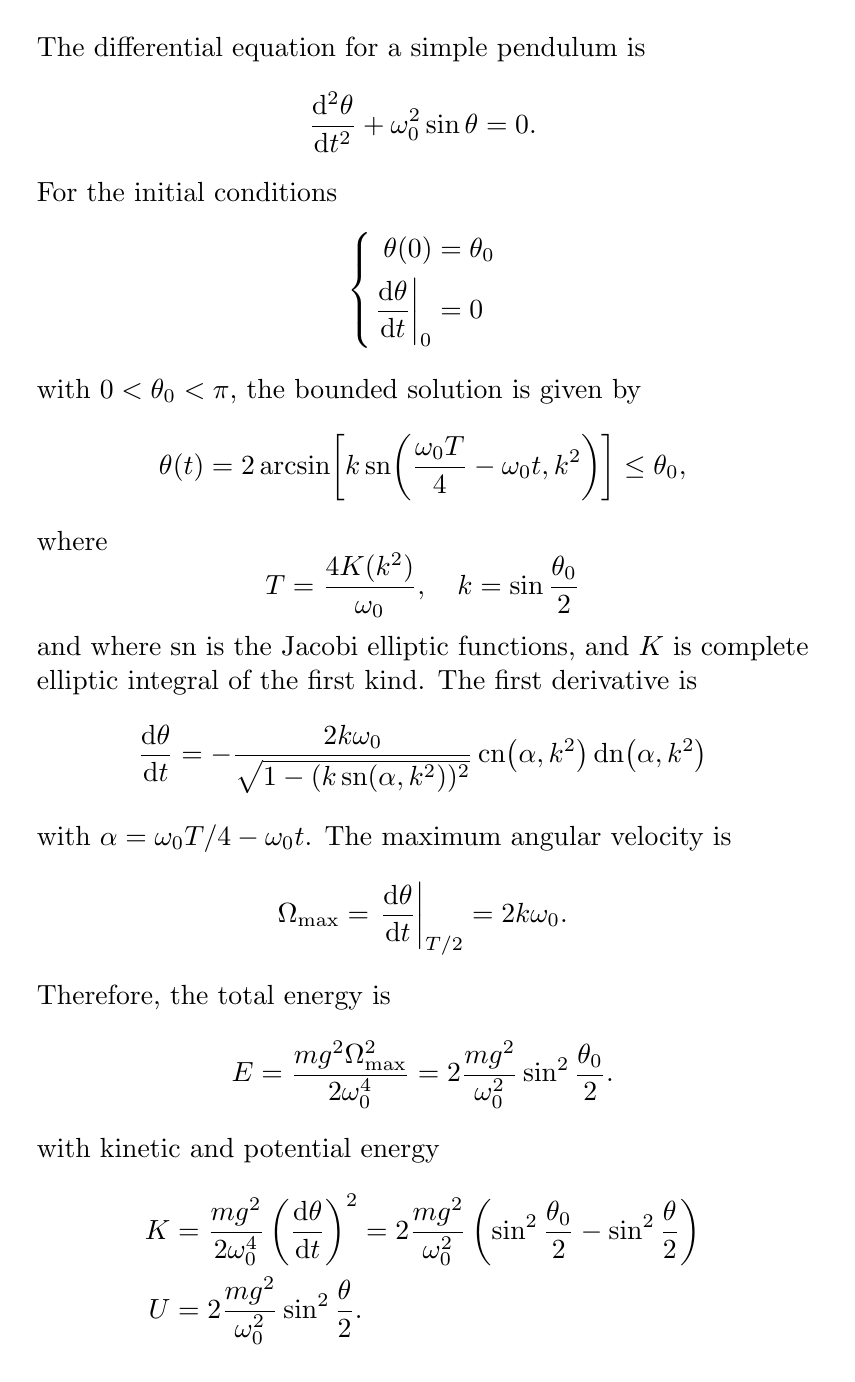
\begin{tikzpicture}[scale=1]
  \message{^^JPendulum equations (closed/bounded)}
  \def\myarg{\left(\alpha,k^2\right)}
  \node[align=left] at (0,0) {
    \begin{minipage}{9.8cm}
      The differential equation for a simple pendulum is
      \begin{equation*}
        \dv{^2\theta}{t^2} + \omega_0^2\sin\theta = 0.
      \end{equation*}
      For the initial conditions
      \begin{equation*}
        \left\{\begin{aligned}
          \theta(0) &= \theta_0\\
          \left.\dv{\theta}{t}\right|_{0} &= 0
        \end{aligned}\right.
      \end{equation*}
      with $0<\theta_0<\pi$,
      the bounded solution is given by
      \begin{equation*}
        \theta(t)
        = 2\arcsin\!\left[k\sn\!\left(\frac{\omega_0T}{4}-\omega_0t,k^2\right)\right]
        \leq \theta_0,
      \end{equation*}
      where
      \begin{equation*}
        %0<\theta_0<\pi,\quad
        T = \frac{4K(k^2)}{\omega_0},\quad
        k = \sin{\frac{\theta_0}{2}}
      \end{equation*}
      and where $\sn$ is the Jacobi elliptic functions,
      and $K$ is complete elliptic integral of the first kind.
      The first derivative is
      \begin{equation*}
        \dv{\theta}{t}
        = -\frac{2 k \omega_0}{\sqrt{1-(k \sn\!\myarg)^2}} \cn\!\myarg\dn\!\myarg
      \end{equation*}
      with $\alpha = \omega_0T/4-\omega_0t$.
      %\begin{equation*}
      %  \alpha = \frac{\omega_0T}{4}-\omega_0t.
      %\end{equation*}
      The maximum angular velocity is
      \begin{equation*}
        \Omega_\mathrm{max} = \left.\dv{\theta}{t}\right|_{T/2} = 2k\omega_0.
      \end{equation*}
      Therefore, the total energy is
      \begin{equation*}
        E = \frac{mg^2\Omega_\mathrm{max}^2}{2\omega_0^4}
          = 2\frac{mg^2}{\omega_0^2}\sin^2\frac{\theta_0}{2}.
      \end{equation*}
      with kinetic and potential energy
      \begin{align*}
        K &= \frac{mg^2}{2\omega_0^4}\left(\dv{\theta}{t}\right)^2
           = 2\frac{mg^2}{\omega_0^2}\left( \sin^2\frac{\theta_0}{2} - \sin^2\frac{\theta}{2} \right) \\
        U &= 2\frac{mg^2}{\omega_0^2}\sin^2\frac{\theta}{2}.
      \end{align*}
     \end{minipage}
  };
\end{tikzpicture}


% PENDULUM EQUATIONS - OPEN TRAJECTORIES
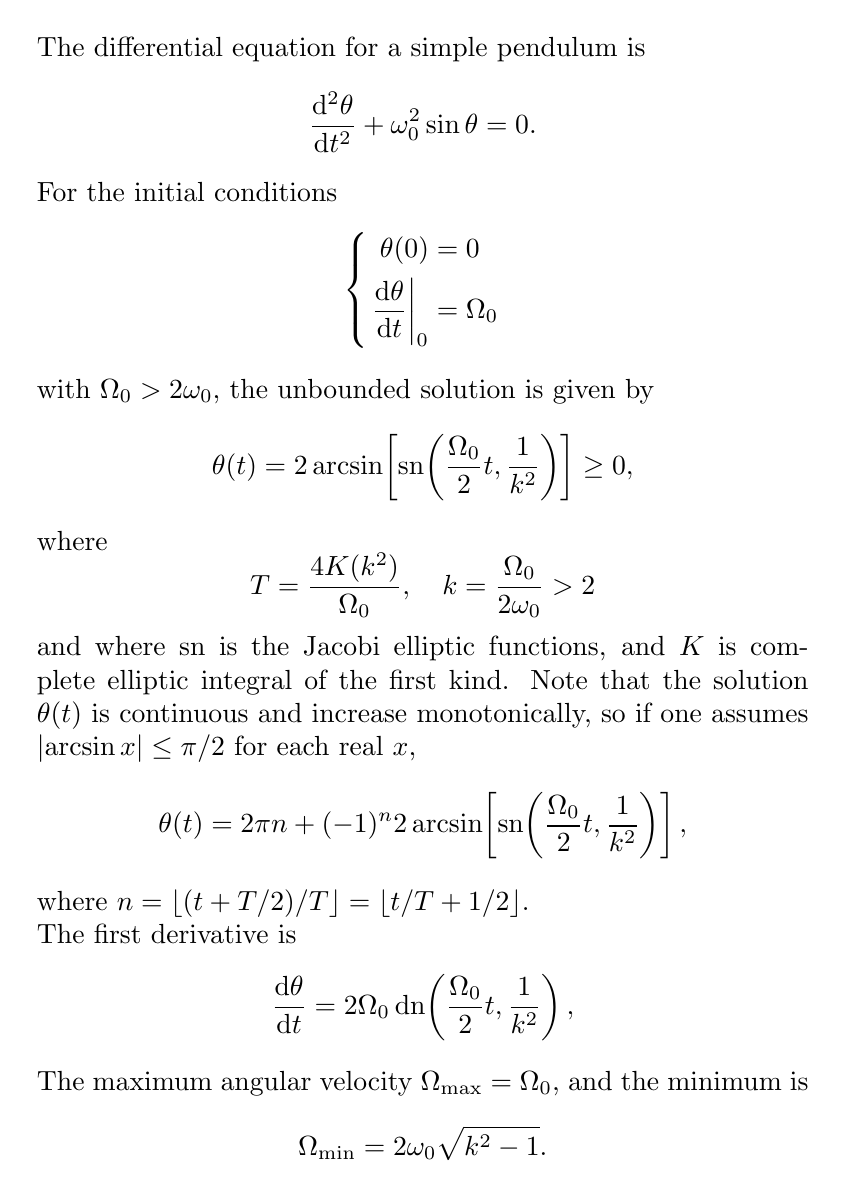
\begin{tikzpicture}[scale=1]
  \message{^^JPendulum equations (open/unbounded)}
  \def\myarg{\left(\frac{\Omega_0}{2}t,\frac{1}{k^2}\right)}
  \node[align=left] at (0,0) {
    \begin{minipage}{9.8cm}
      The differential equation for a simple pendulum is
      \begin{equation*}
        \dv{^2\theta}{t^2} + \omega_0^2\sin\theta = 0.
      \end{equation*}
      For the initial conditions
      \begin{equation*}
        \left\{\begin{aligned}
          \theta(0) &= 0 \\
          \left.\dv{\theta}{t}\right|_{0} &= \Omega_0 %> 2\omega_0
        \end{aligned}\right.
      \end{equation*}
      with $\Omega_0 > 2\omega_0$,
      the unbounded solution is given by
      \begin{equation*}
        \theta(t)
        = 2\arcsin\!\left[\sn\!\myarg\right]
        \geq 0,
      \end{equation*}
      where
      \begin{equation*}
        %\Omega_0 > 2\omega_0,\quad
        T = \frac{4K(k^2)}{\Omega_0},\quad
        k = \frac{\Omega_0}{2\omega_0} > 2
      \end{equation*}
      and where sn is the Jacobi elliptic functions,
      and $K$ is complete elliptic integral of the first kind.
      Note that the solution $\theta(t)$ is continuous and increase monotonically,
      so if one assumes $\abs{\arcsin x}\leq\pi/2$ for each real $x$,
      \begin{equation*}
        \theta(t)
        = 2\pi n + (-1)^n 2\arcsin\!\left[\sn\!\myarg\right],
      \end{equation*}
      where $n=\lfloor(t+T/2)/T\rfloor=\lfloor t/T+1/2\rfloor$.\\
      The first derivative is
      \begin{equation*}
        \dv{\theta}{t} = 2\Omega_0\dn\!\myarg,
      \end{equation*}
      The maximum angular velocity $\Omega_\mathrm{max}=\Omega_0$,
      and the minimum is
      \begin{equation*}
        \Omega_\mathrm{min} = 2\omega_0\sqrt{k^2-1}.
      \end{equation*}
    \end{minipage}
  };
\end{tikzpicture}


\end{document}